\begin{figure}[H]
    \center
    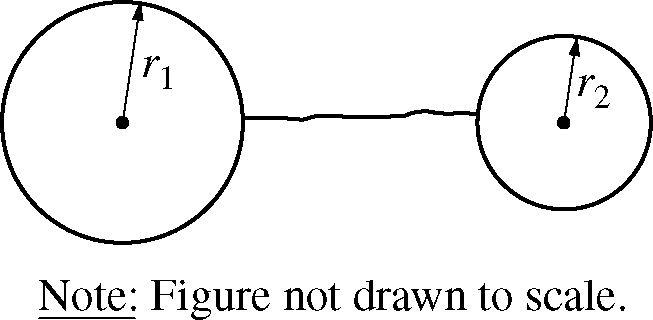
\includegraphics[scale=0.25]{images/img-006-014.png}
\end{figure}

% Multiple Choice Question 14
\begin{questions}\setcounter{question}{13}\question
A metal sphere with radius $r_{1}$ has a total electric charge of magnitude $q$. An uncharged metal sphere with radius $r_{2}$ (with $r_{1}>r_{2}$) is then connected by a wire to the first sphere, as illustrated above. The separation of the spheres is much greater than the radius of either sphere. When equilibrium is reached, the spheres will have

\begin{choices}
\choice charges on their surfaces of equal magnitude and the same sign
\choice charges on their surfaces of equal magnitude and opposite sign
\choice equal electric fields at their surfaces
\choice equal capacitances
\choice equal electric potentials
\end{choices}\end{questions}

